% Autor: Leonhard Segger, Alexander Neuwirth
% Datum: 2017-10-30
\documentclass[
	% Papierformat
	a4paper,
	% Schriftgröße (beliebige Größen mit „fontsize=Xpt“)
	12pt,
	% Schreibt die Papiergröße korrekt ins Ausgabedokument
	pagesize,
	% Sprache für z.B. Babel
	ngerman
]{scrartcl}

% Achtung: Die Reihenfolge der Pakete kann (leider) wichtig sein!
% Insbesondere sollten (so wie hier) babel, fontenc und inputenc (in dieser
% Reihenfolge) als Erstes und hyperref und cleveref (Reihenfolge auch hier
% beachten) als Letztes geladen werden!

% Silbentrennung etc.; Sprache wird durch Option bei \documentclass festgelegt
\usepackage{babel}
% Verwendung der Zeichentabelle T1 (Sonderzeichen etc.)
\usepackage[T1]{fontenc}
% Legt die Zeichenkodierung der Eingabedatei fest, z.B. UTF-8
\usepackage[utf8]{inputenc}
% Schriftart
\usepackage{lmodern}
% Zusätzliche Sonderzeichen
\usepackage{textcomp}

% Mathepaket (intlimits: Grenzen über/unter Integralzeichen)
\usepackage[intlimits]{amsmath}
% Ermöglicht die Nutzung von \SI{Zahl}{Einheit} u.a.
\usepackage{siunitx}
% Zum flexiblen Einbinden von Grafiken (\includegraphics)
\usepackage{graphicx}
% Abbildungen im Fließtext
\usepackage{wrapfig}
% Abbildungen nebeneinander (subfigure, subtable)
\usepackage{subcaption}
% Funktionen für Anführungszeichen
\usepackage{csquotes}
% Zitieren, Bibliographie
\usepackage{biblatex}


% Zur Darstellung von Webadressen
\usepackage{url}
%chemische Formeln
\usepackage[version=4]{mhchem}
% siunitx: Deutsche Ausgabe, Messfehler getrennt mit ± ausgeben
\usepackage{floatrow}
\floatsetup[table]{capposition=top}
\usepackage{float}
% Verlinkt Textstellen im PDF-Dokument
\usepackage[unicode]{hyperref}
% "Schlaue" Referenzen (nach hyperref laden!)
\usepackage{cleveref}
\sisetup{
	locale=DE,
	separate-uncertainty
}
%\bibliography{6Mi_M3_29-11-2017_References}

\begin{document}
	
	\begin{titlepage}
		\centering
		{\scshape\LARGE Versuchsbericht zu \par}
		\vspace{1cm}
		{\scshape\huge EX - Titel \par} %TODO Anpasen
		\vspace{2.5cm}
		{\LARGE Gruppe 6Mi \par}
		\vspace{0.5cm}
		
		{\large Alexander Neuwirth (E-Mail: a\_neuw01@wwu.de) \par}
		{\large Leonhard Segger (E-Mail: l\_segg03@uni-muenster.de) \par}
		\vfill
		
		durchgeführt am DD.MM.JJJJ\par %TODO Anpassen
		betreut von\par
		{\large VN NN} %TODO Anpassen
		
		\vfill
		
		{\large \today\par}
	\end{titlepage}
	\tableofcontents
	\newpage

	%TODO mehr TODO in Default	

	\section{Kurzfassung}
	%TODO Hypothese	und deren Ergebnis
	%TODO Ergebnisse, auch Zahlen, mindestens wenn's halbwegs Sinn ergibt
	%TODO Was wurde gemacht
	
	\section{Methoden}
	%TODO Bilder von der Website klauen
	
	\section{Ergebnisse und Diskussion}
	%TODO Datenanalyse -> Überschrift?
	%TODO Unsicherheiten
	

	\subsection{Beobachtung}
	\subsection{Strom-Spannungs-Charakteristiken}
	Im Folgenden ergibt sich der Fehler der Strom- und Spannungsmessung aus der Unsicherheit durch die Digitalanzeige der verwendeten Multimeter (also rechteckige WDF).
	Da in unterschiedlichen Skalen gemessen wurde, wurde hierfür jeweils die Unsicherheit des Messwerts mit der größten Skala verwendet.
	Die Abhängigkeit der Stromstärke von der Spannung der verwendeten Diode in Durchlassrichtung wurde in \cref{Diode} dargestellt.
	\begin{figure}[H]
		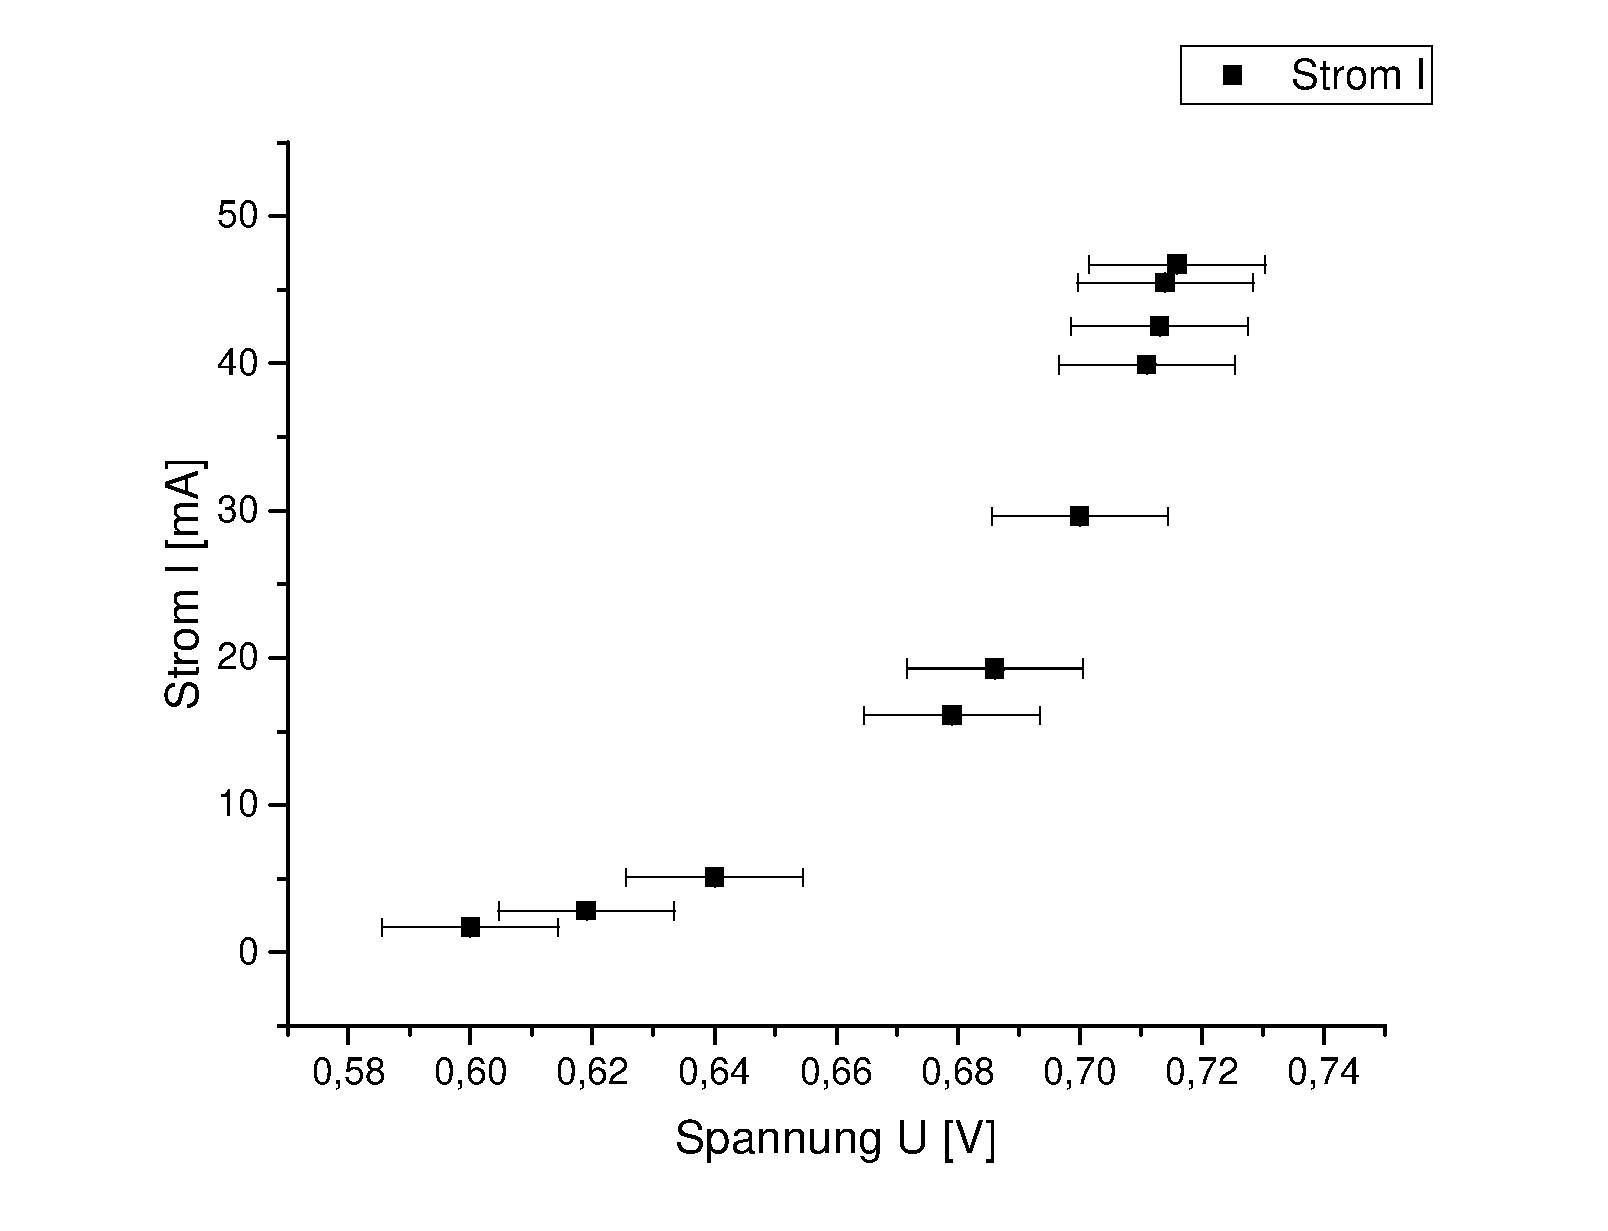
\includegraphics[width=0.7\textwidth]{Diode}
		\centering
		\caption{Hier ist die Stromstärke  gegen die Spannung bei Betrieb einer Diode aufgetragen. Die Unsicherheit in y-Richtung ist kleiner als die Symbolgröße.}
		\label{Diode}
		\centering
	\end{figure} 
	In \crefrange{Zener_Durch}{Zener_Sperr} wurden die experimentell ermittelten Kennlinien der Zenerdiode in Durchfluss- und Sperrrichtung aufgetragen.
	\begin{figure}[H]
		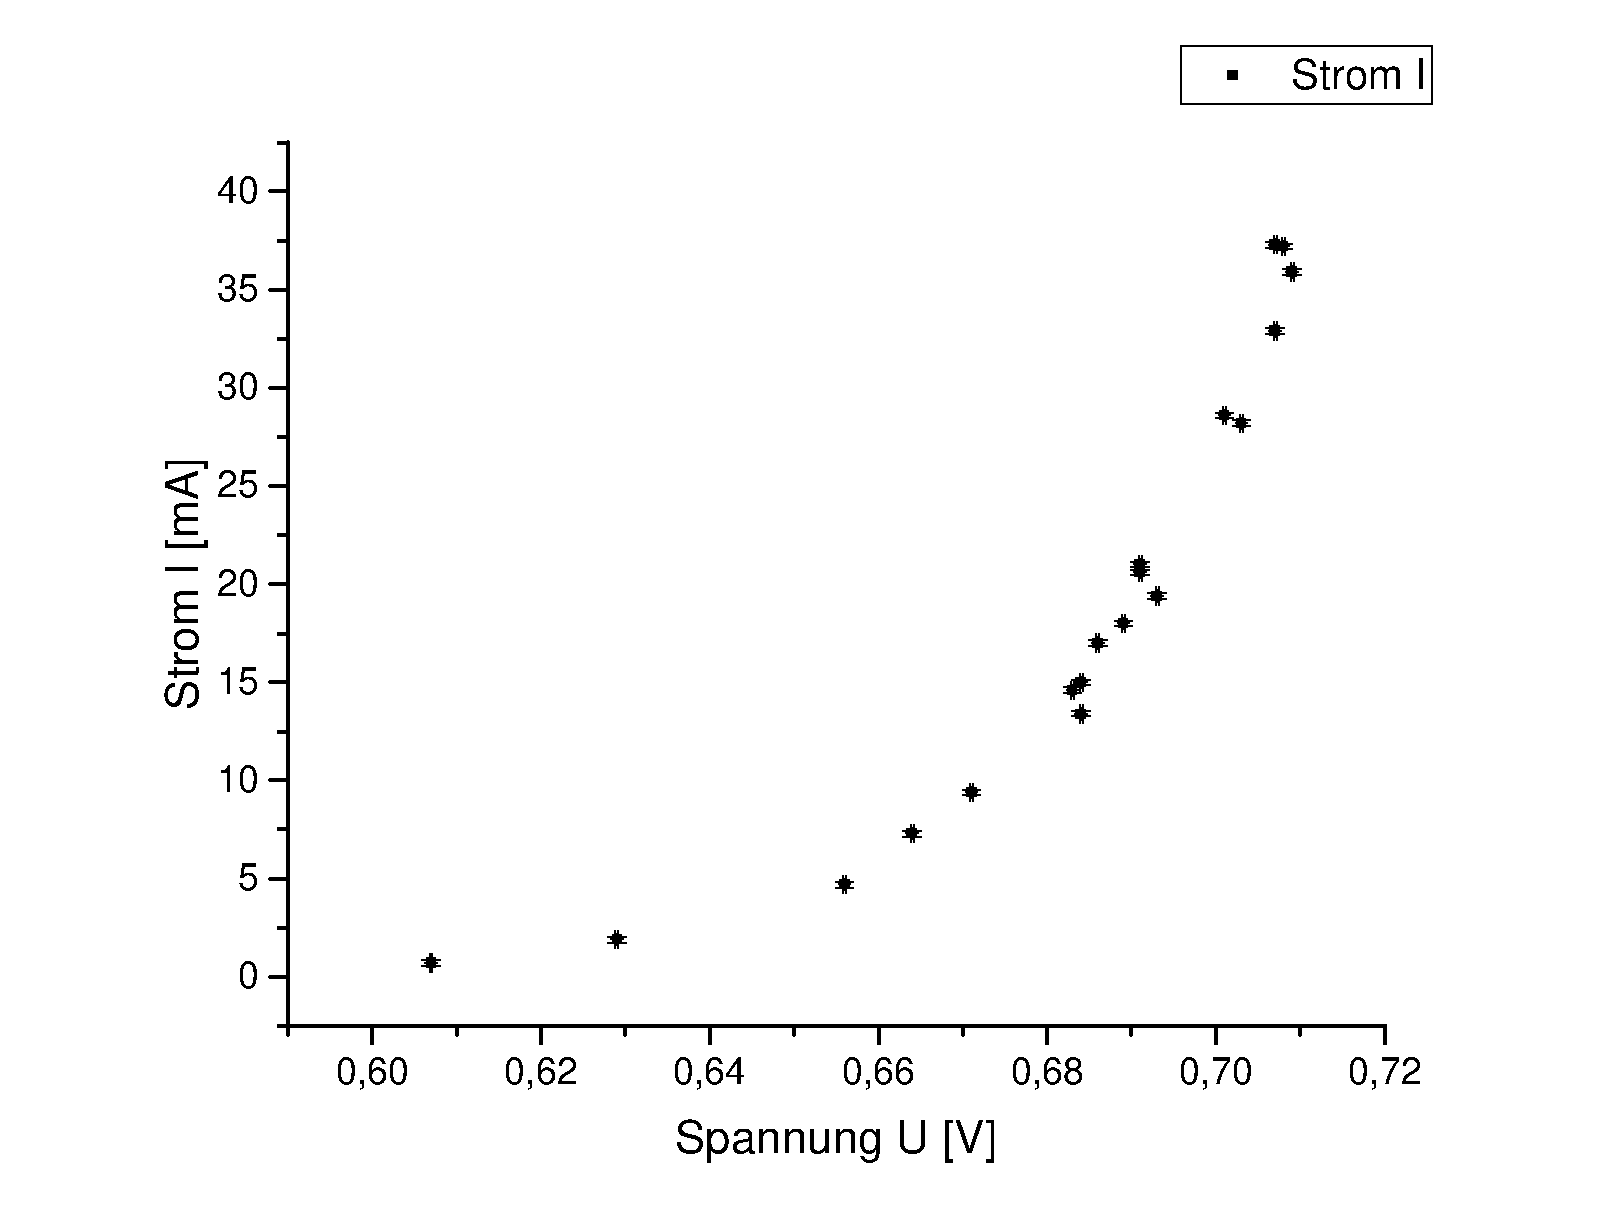
\includegraphics[width=0.7\textwidth]{Zener_Durch}
		\centering
		\caption{Hier ist die Stromstärke  gegen die Spannung bei Betrieb einer Zenerdiode in Durchflussrichtung aufgetragen. Die Unsicherheit ist kleiner als die Symbolgröße.}
		\label{Zener_Durch}
		\centering
	\end{figure}
	\begin{figure}[H]
		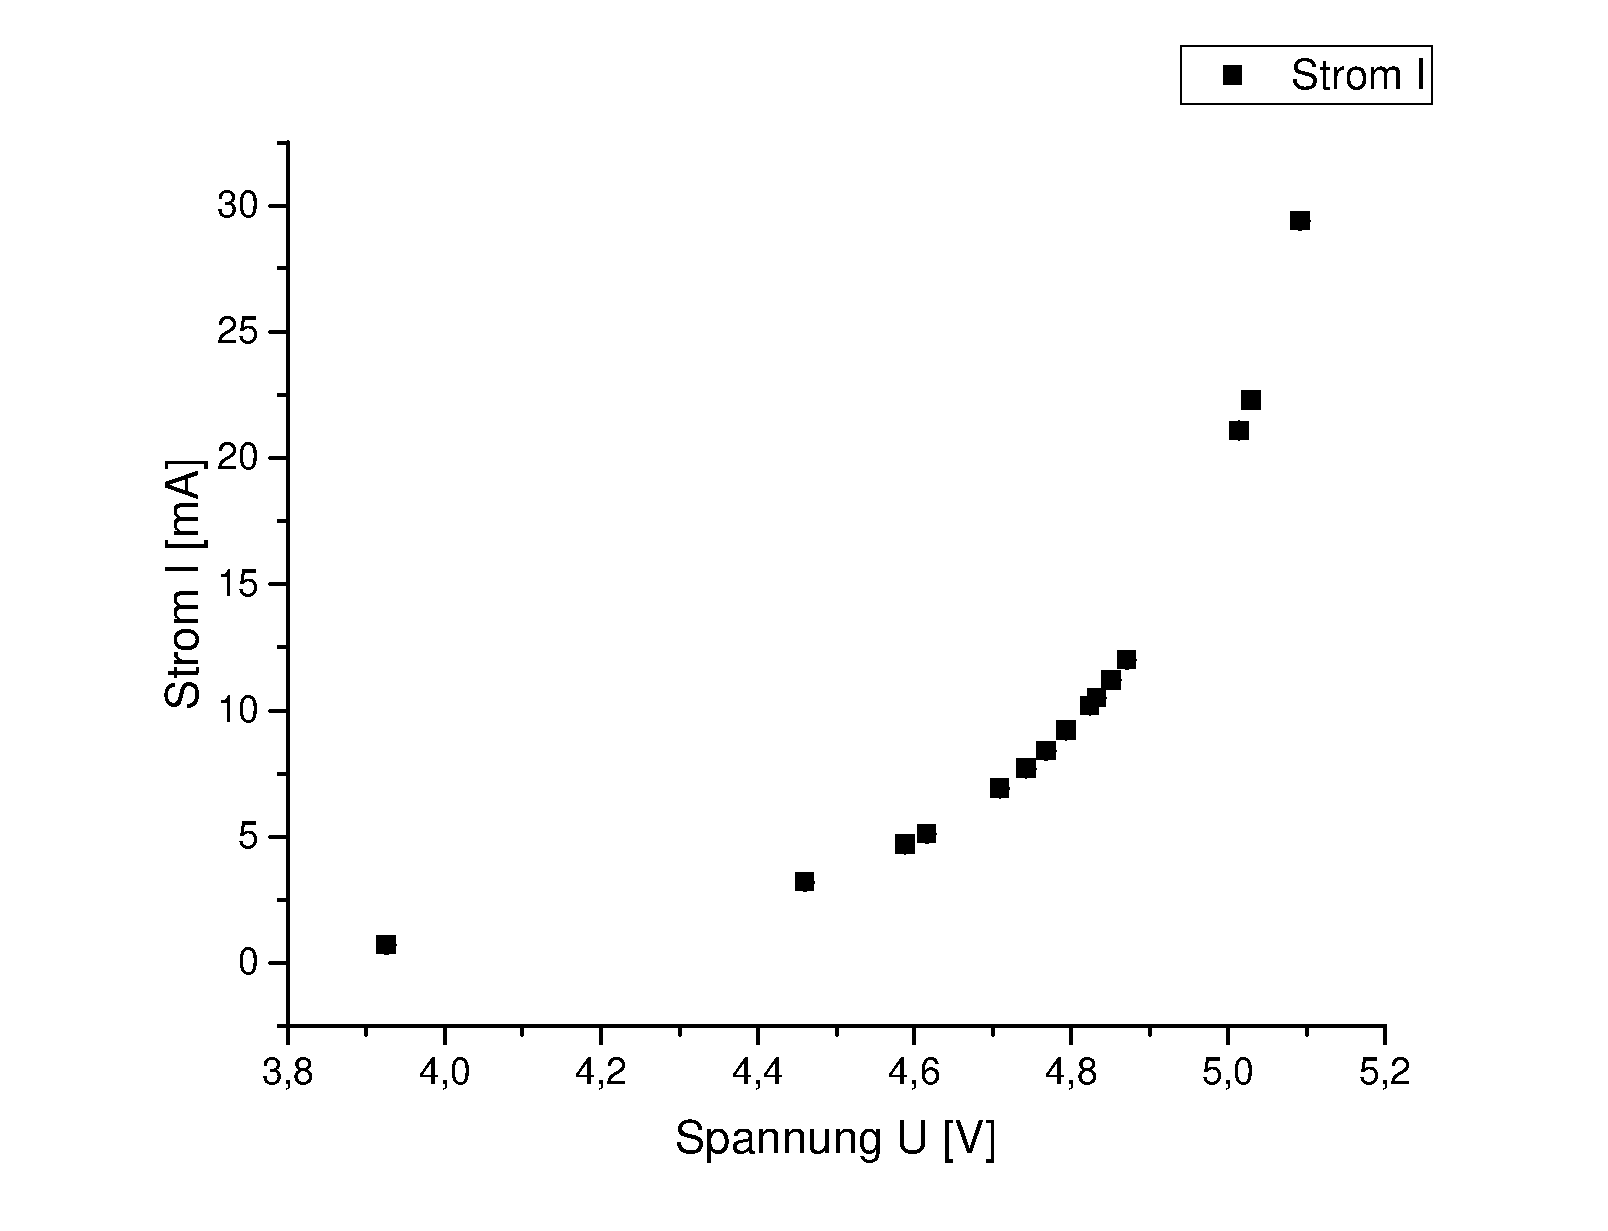
\includegraphics[width=0.7\textwidth]{Zener_Sperr}
		\centering
		\caption{Hier ist die Stromstärke gegen die Spannung bei Betrieb einer Zenerdiode in Sperrrichtung aufgetragen. Die Unsicherheit ist kleiner als die Symbolgröße.}
		\label{Zener_Sperr}
		\centering
	\end{figure}
	Als nächstes wurde die Glühlampe untersucht.
	Die zugehörige Kennlinie ist in \cref{Glueh_Kenn} zu finden, während in \cref{Glueh_Wider} der Widerstand gegen die Spannung aufgetragen wurde.
	Dazu wurde das Gesetz
	\begin{equation*}
		R=\frac{U}{I}
	\end{equation*}
	verwendet.
	Die Unsicherheit wurde gemäß \cref{Partielle_Unsicherheiten} berechnet.
	Wenn man die nahezu linear verlaufenden Werte unter \SI{1,5}{V} in \cref{Glueh_Wider} extrapoliert, erhält man für $V=0$ also ohne Stromfluss und damit bei Zimmertemperatur einen Widerstand von \SI{25\pm2,1}{\ohm} (nach oben abgeschätzte Ableseunsicherheit mit dreieckiger WDF).
	\begin{equation}
	u(y) = \sqrt{  \sum_{i=0}^{N} \left( \frac{\partial y}{\partial x_i}u(x_i)\right)^2  }
	\label{Partielle_Unsicherheiten}
	\end{equation}
	\begin{figure}[H]
		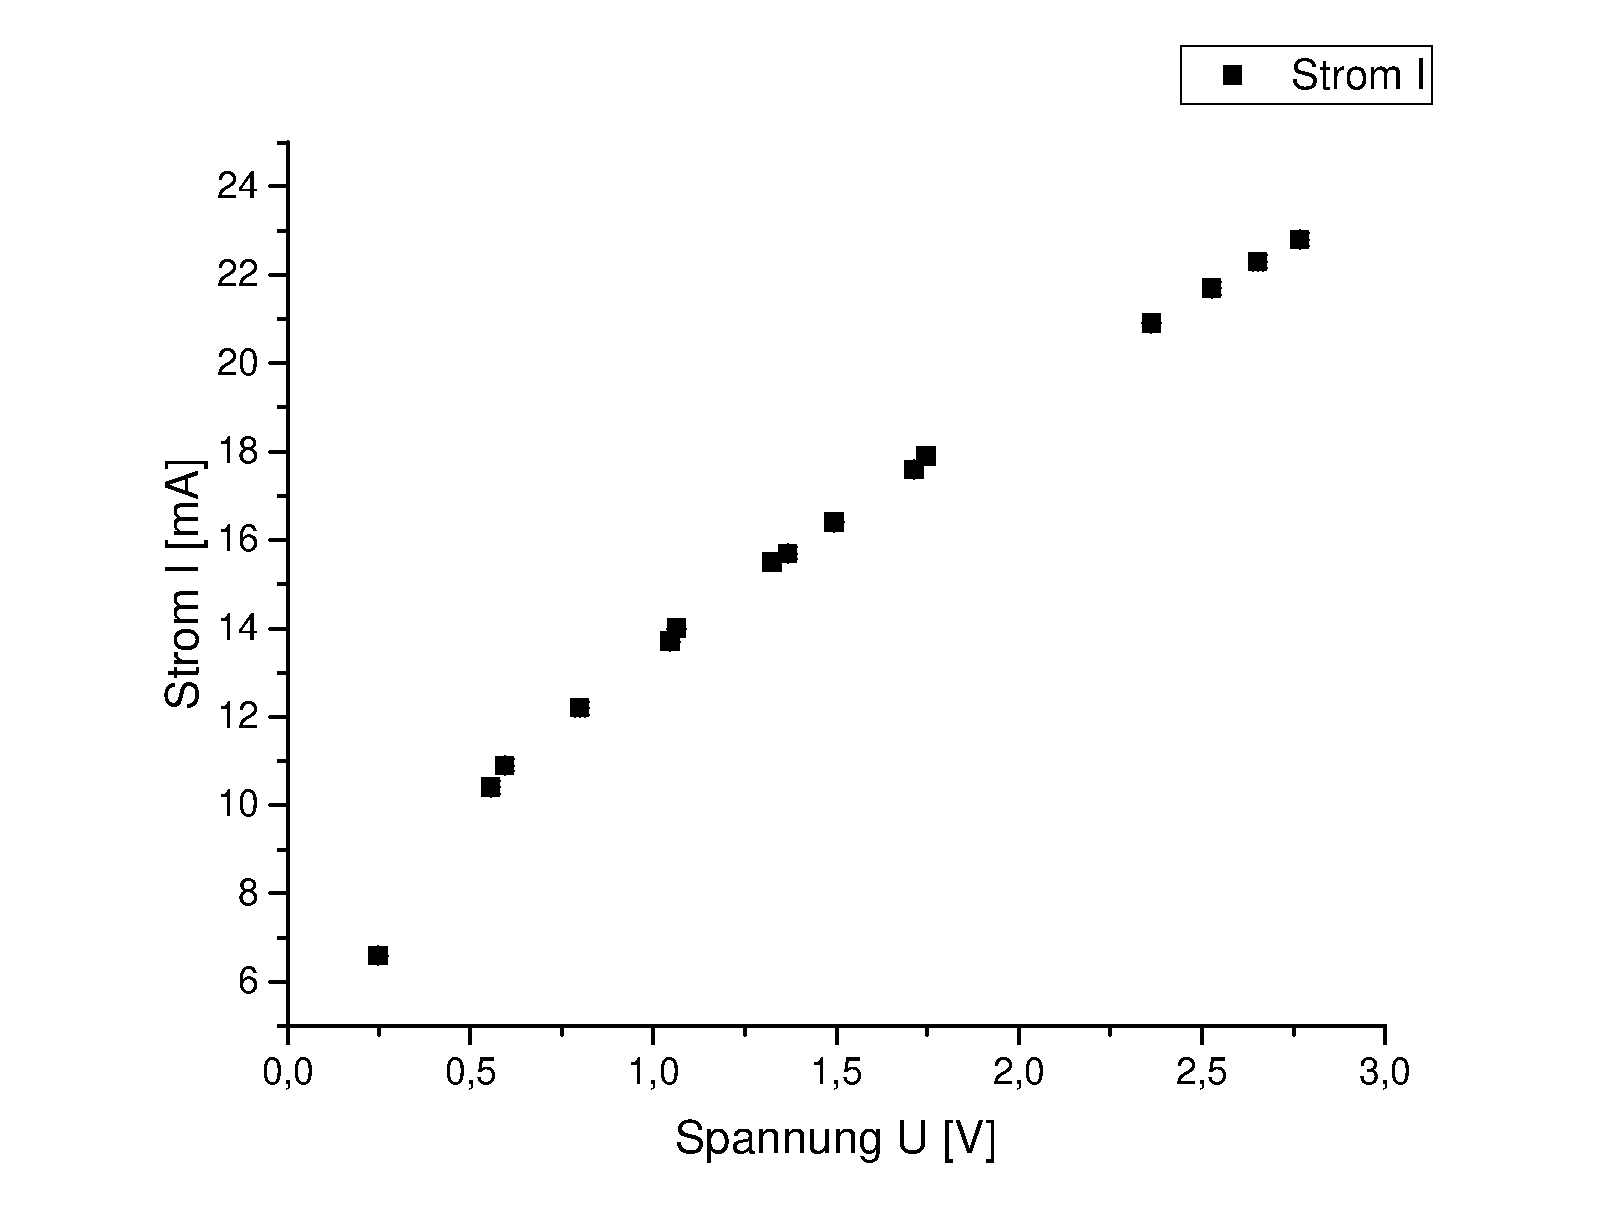
\includegraphics[width=0.7\textwidth]{Glueh_Kenn}
		\centering
		\caption{Hier ist die Stromstärke gegen die Spannung bei Betrieb einer Glühlampe aufgetragen. Die Unsicherheit ist kleiner als die Symbolgröße.}
		\label{Glueh_Kenn}
		\centering
	\end{figure}
	\begin{figure}[H]
		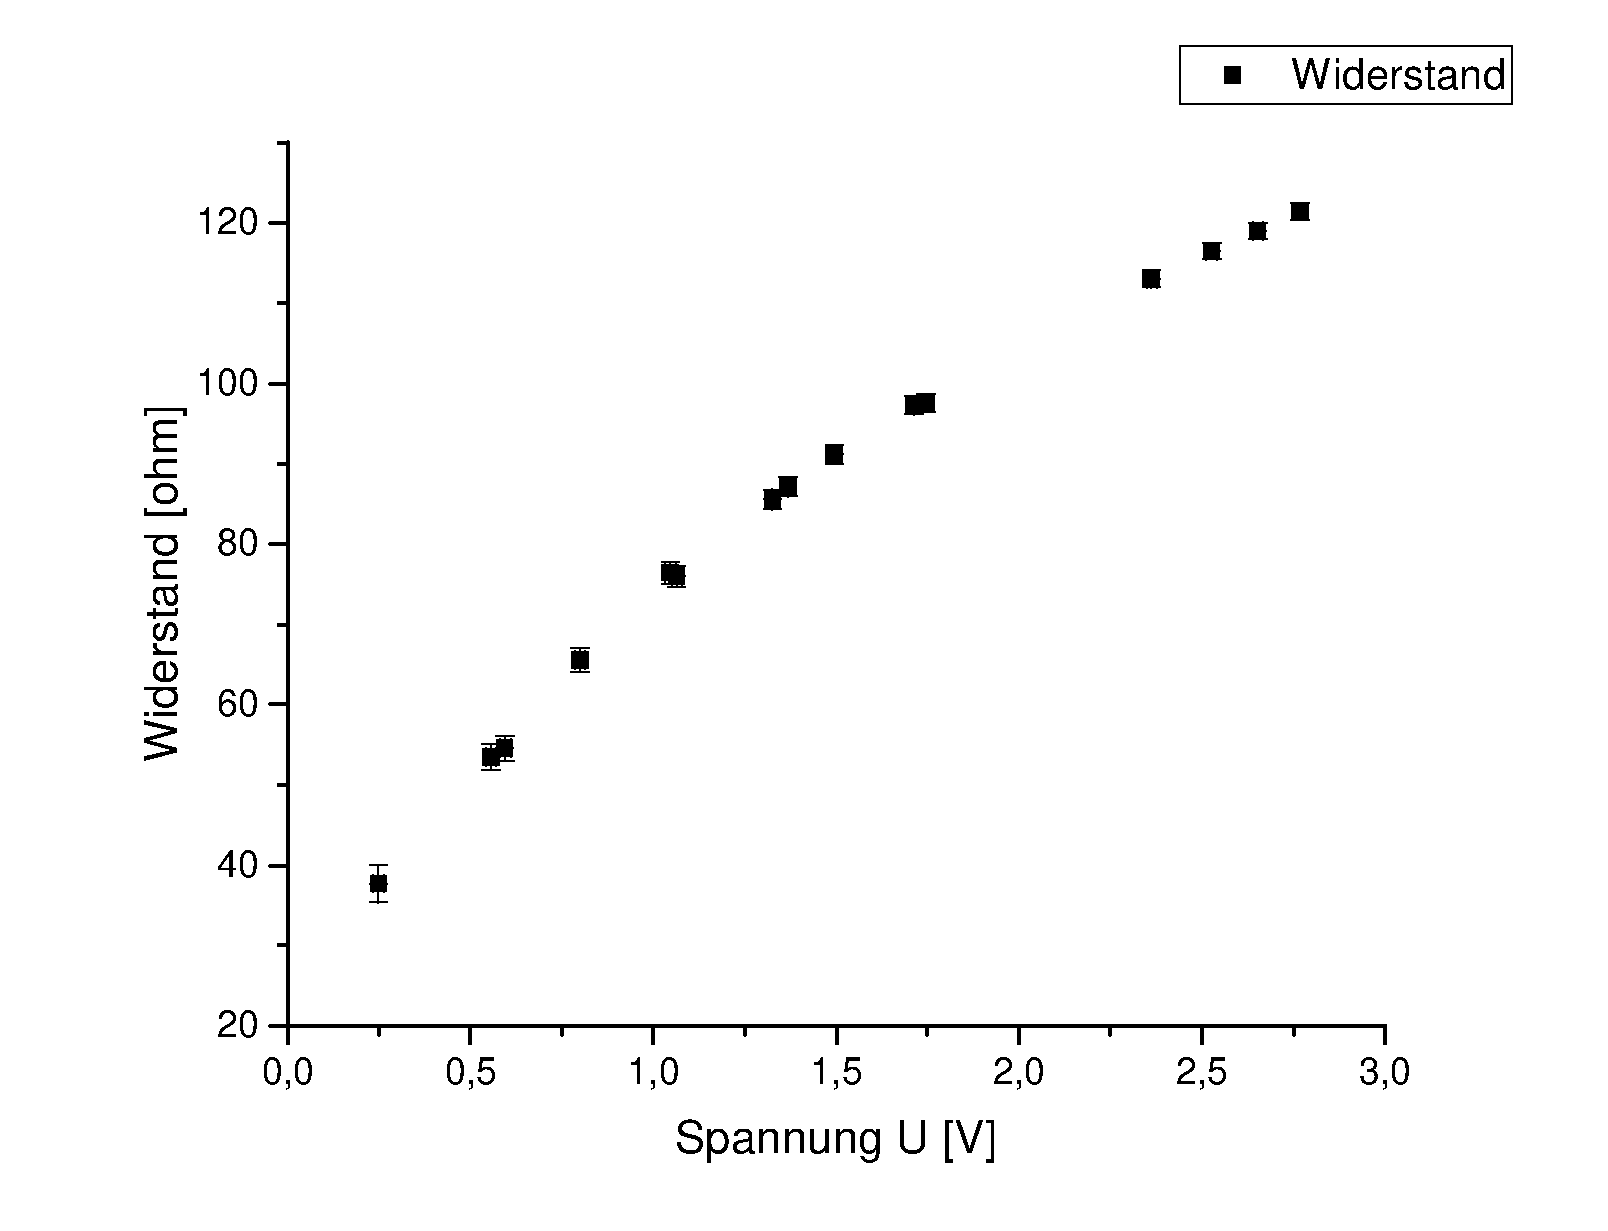
\includegraphics[width=0.7\textwidth]{Glueh_Wider}
		\centering
		\caption{Hier ist der Widerstand gegen die Spannung bei Betrieb einer Glühlampe aufgetragen. Die Unsicherheit ist kleiner als die Symbolgröße.}
		\label{Glueh_Wider}
		\centering
	\end{figure}
	Die aufgenommenen Kennlinie des NTC-Widerstands ist in \cref{ntc} dargestellt.
	\begin{figure}[H]
		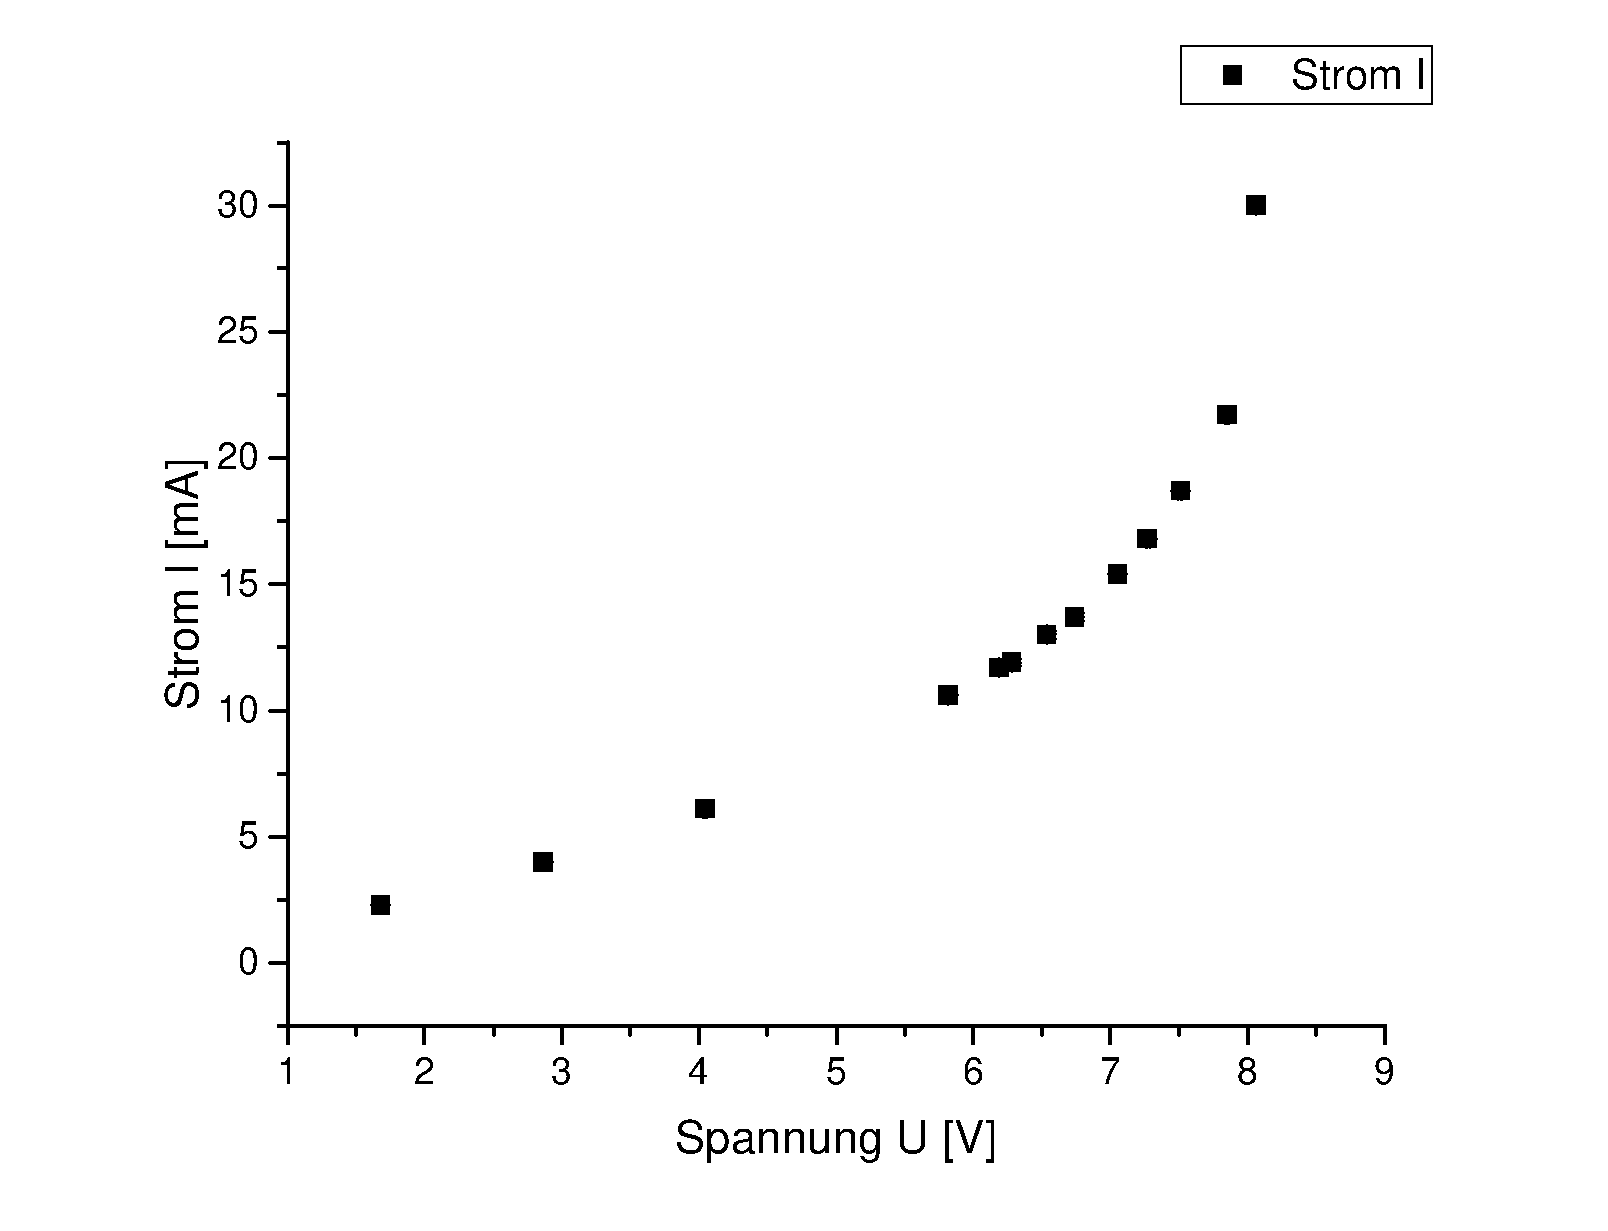
\includegraphics[width=0.7\textwidth]{ntc}
		\centering
		\caption{Hier ist der Widerstand gegen die Spannung bei Betrieb eines NTC-Widerstandes aufgetragen. Die Unsicherheit ist kleiner als die Symbolgröße.}
		\label{ntc}
		\centering
	\end{figure}
	Zuletzt soll die Glimmlampe betrachtet werden.
	Dazu wurde in \crefrange{glimm_steig}{glimm_fall} die Kennlinie für steigende bzw. fallende Spannungen dargestellt.
	Hieraus kann die Zünd- und Löschspannung der vorliegenden Glimmlampe bestimmt werden.
	Dazu wurde im Fall der Zündspannung der höchste Messwert gewählt, bei dem die Glimmlampe noch nicht zündete und das Messintervall als Fehler angenommen (mit rechteckiger WDF).
	Analog wurde die Löschspannung aus dem niedrigsten Messwert, bei dem die Glimmlampe noch leuchtete, bestimmt.
	Dies ergibt eine Zündspannung von \SI{105\pm3,8}{V} und eine Löschspannung von \SI{84\pm 0,7}{V}.
	
	\begin{figure}[H]
		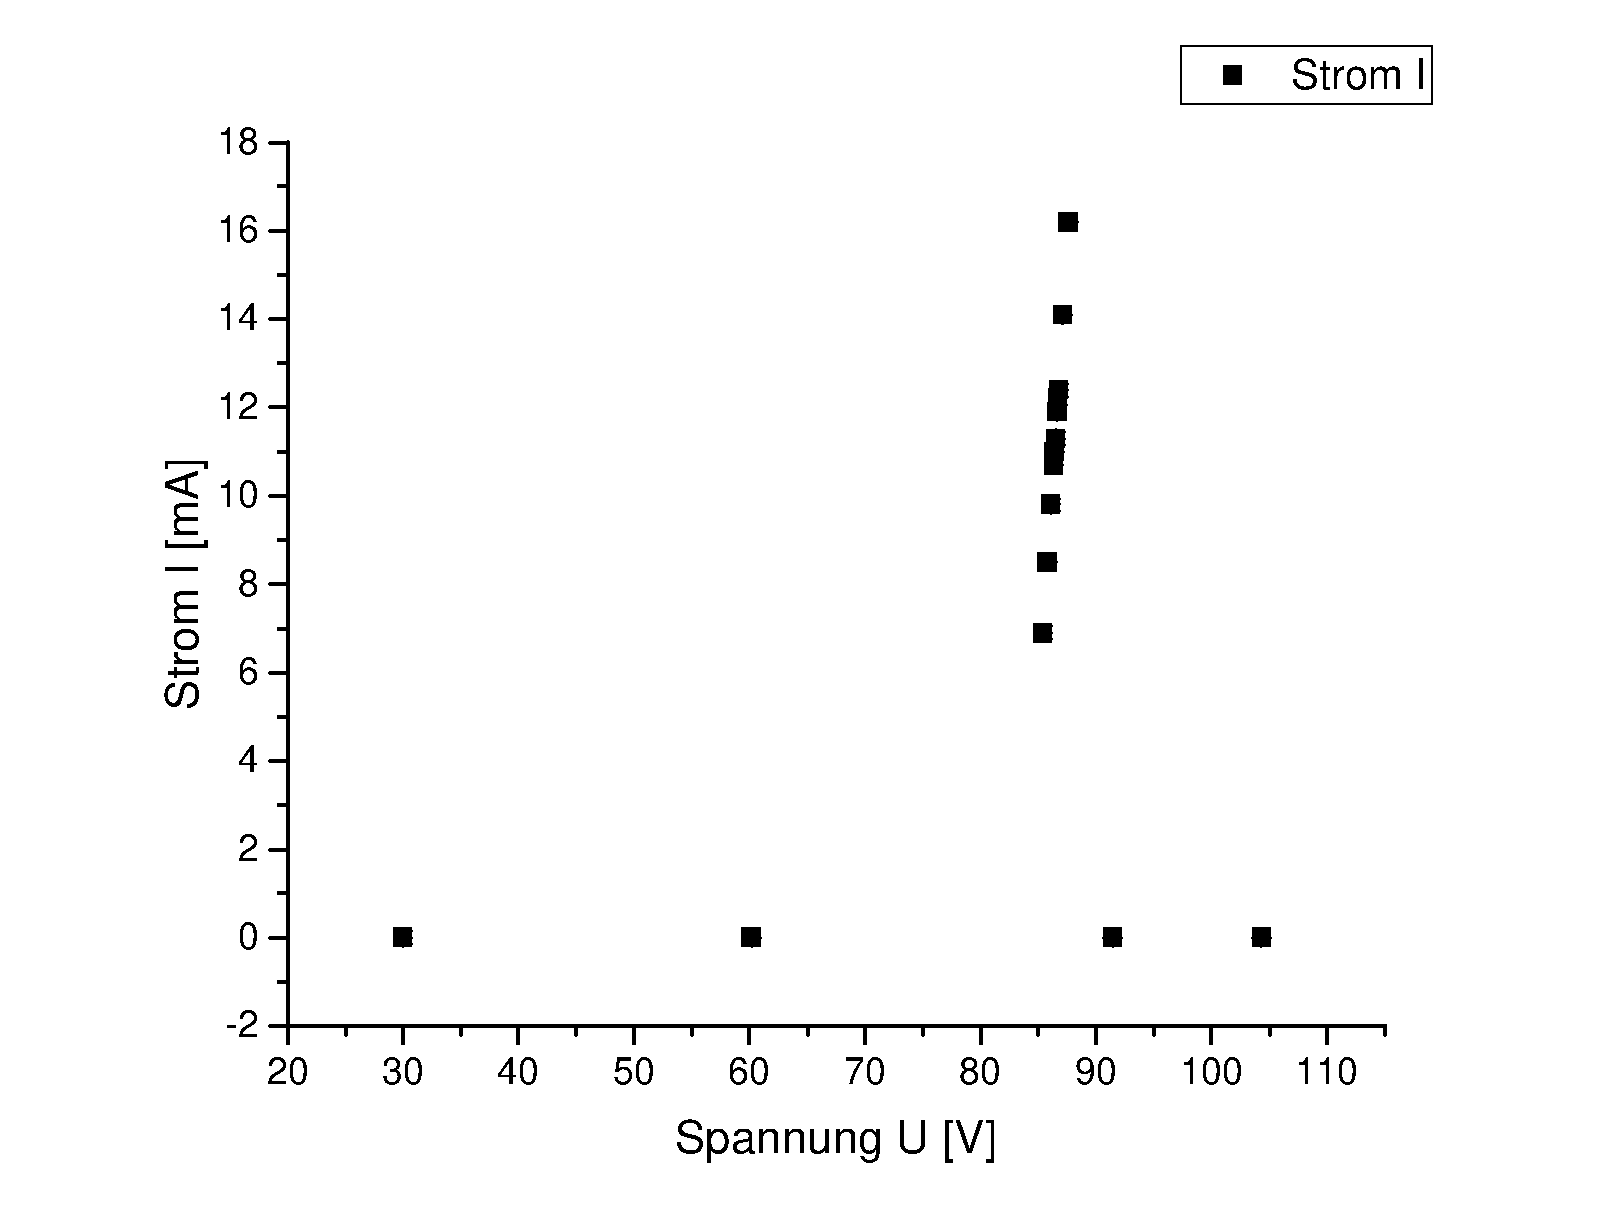
\includegraphics[width=0.7\textwidth]{glimm_steig}
		\centering
		\caption{Hier ist der Widerstand gegen die Spannung bei Betrieb einer Glimmlampe mit steigender Spannung aufgetragen. Die Unsicherheit ist kleiner als die Symbolgröße. Die Messwerte bei $I=0$ sind die Spannungen, bei denen die Glimmlampe noch nicht zündete.}
		\label{glimm_steig}
		\centering
	\end{figure}
\begin{figure}[H]
	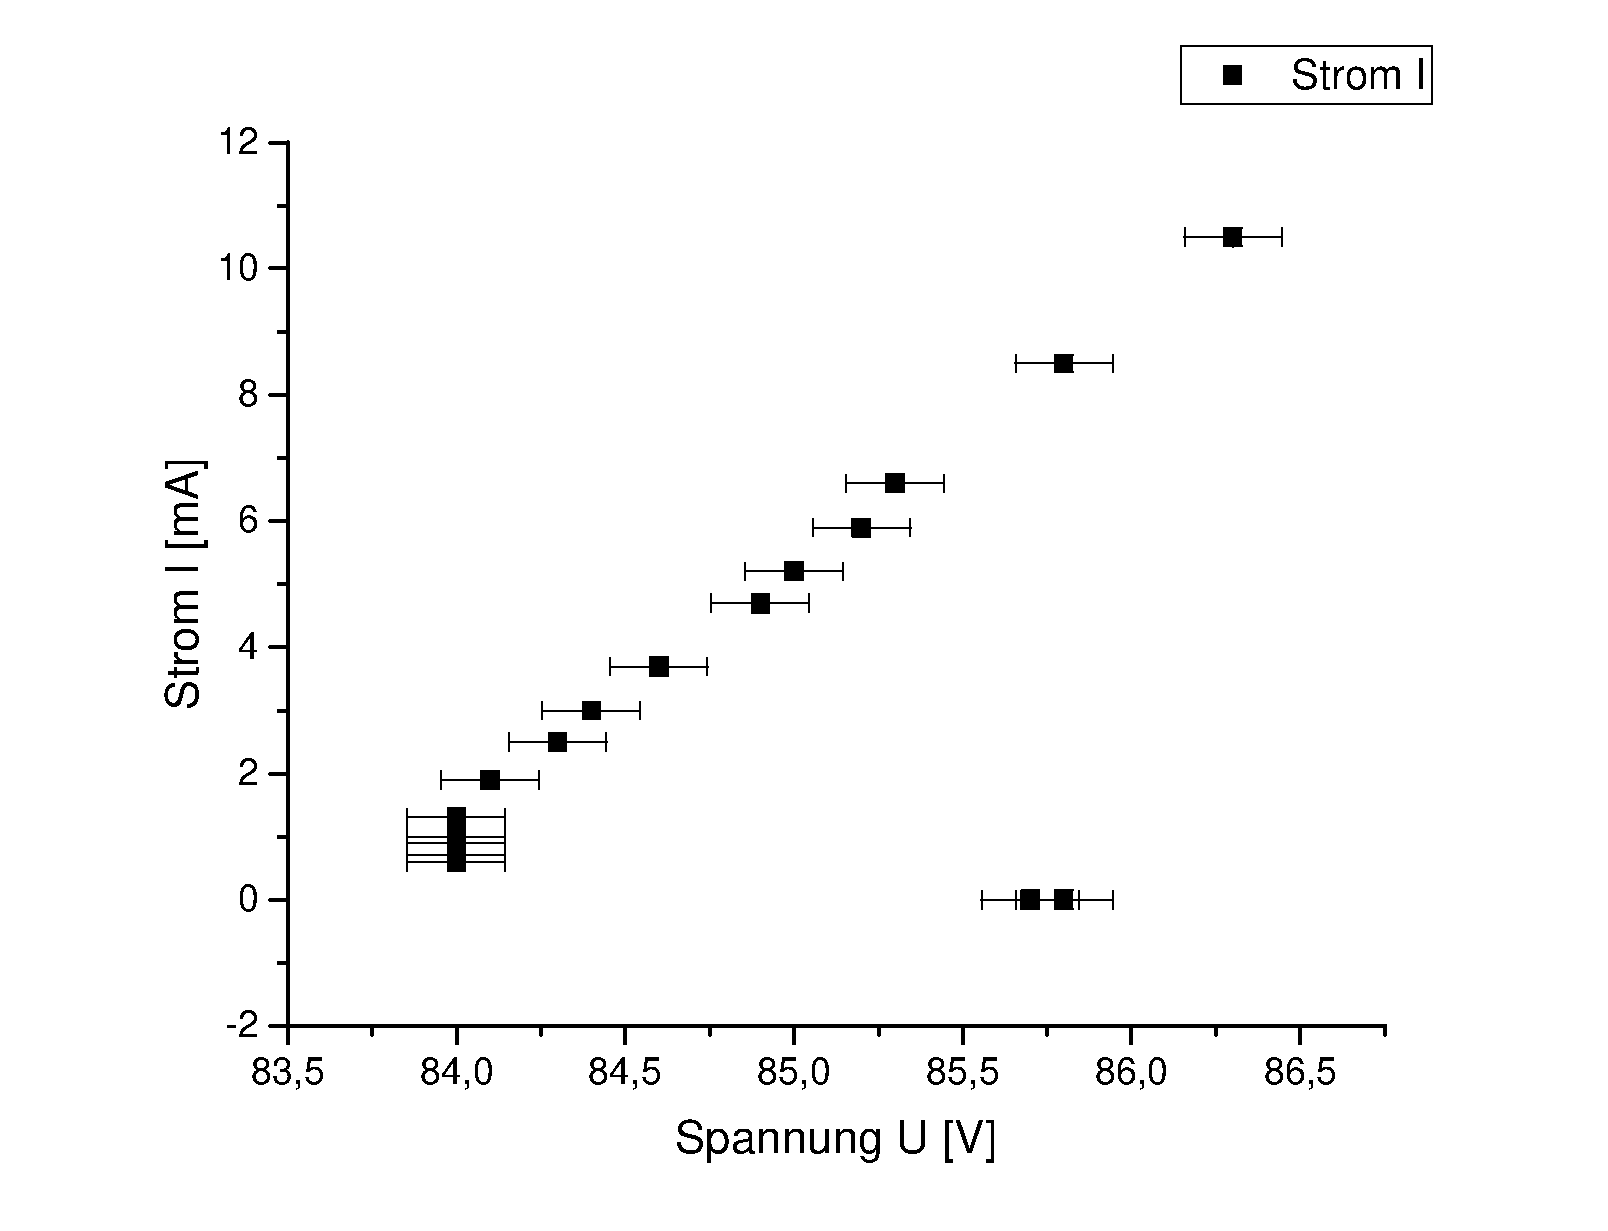
\includegraphics[width=0.7\textwidth]{glimm_fall}
	\centering
	\caption{Hier ist der Widerstand gegen die Spannung bei Betrieb einer Glimmlampe mit sinkender Spannung aufgetragen. Die Unsicherheit in y-Richtung ist kleiner als die Symbolgröße. Die Messwerte bei $I=0$ sind die Spannungen, bei denen die Glimmlampe erloschen war.}
	\label{glimm_fall}
	\centering
\end{figure}
	\subsection{Diskussion}
	%TODO Bezug/Nutzten oder sonst was
	%TODO auch hier die Hypothese wiederholen
	
	\section{Schlussfolgerung}
	%TODO Rückgriff auf Hypothese und drittes Nennen dieser
	
	%TODO Quellen zitieren, Websiten mit Zugriffsdatum
	%TODO Verweise auf das Laborbuch (sind erlaubt)
	%TODO Tabelle + Bilder mit Beschriftung
	%\printbibliography
\end{document}
